% !TEX program = xelatex
% The Decider's Dilemma: Computability Limits of Autonomous AI Security Agents
% Charalampos Nadiotis, 2026
%
% Build:  xelatex main.tex ; xelatex main.tex   (run twice for refs)
% All numeric results are injected from results/macros.tex, which is produced
% by experiment.py. Do not hand-edit numbers.
\documentclass[11pt]{article}

\usepackage{amsmath,amsthm,amssymb}
\usepackage{fontspec}            % XeLaTeX font selection
\setmainfont{Latin Modern Roman}[SmallCapsFont={Latin Modern Roman Caps}]
\setmonofont{Latin Modern Mono}

\usepackage[a4paper,margin=1in]{geometry}
\usepackage{microtype}
\usepackage{graphicx}
\usepackage{booktabs}
\usepackage{caption}
\usepackage{subcaption}
\usepackage{xcolor}
\usepackage{enumitem}
\usepackage[hidelinks]{hyperref}
\usepackage{cleveref}

\definecolor{navy}{HTML}{1B4965}
\hypersetup{colorlinks=true, linkcolor=navy, citecolor=navy, urlcolor=navy}

\theoremstyle{plain}
\newtheorem{theorem}{Theorem}
\newtheorem{proposition}{Proposition}
\newtheorem{corollary}{Corollary}
\theoremstyle{definition}
\newtheorem{definition}{Definition}

% ---- experiment-generated numbers ----
\newcommand{\expQ}{6}
\newcommand{\expN}{4,000}
\newcommand{\expBmax}{20,000}
\newcommand{\expNhalt}{738}
\newcommand{\expNnonhalt}{3,262}
\newcommand{\expHaltPct}{18.4}
\newcommand{\expNonhaltPct}{81.5}
\newcommand{\expMedianHalt}{2}
\newcommand{\expHaltPtail}{13}
\newcommand{\expMaxHalt}{32}
\newcommand{\expDetN}{3}
\newcommand{\expEvaderM}{500}
\newcommand{\expEvTrials}{1,500}
\newcommand{\expEvRate}{100.0}
\newcommand{\expSbN}{20,000}
\newcommand{\expSbBenignPct}{40.0}
\newcommand{\expSbMedDelay}{63}
\newcommand{\expSbDelayTail}{147,488}
\newcommand{\expSbWindow}{1,000}
\newcommand{\expSbRecall}{70.0}
\newcommand{\expSbFnr}{30.0}


\title{\textbf{The Decider's Dilemma:\\ Computability Limits of Autonomous AI Security Agents}}
\author{Charalampos Nadiotis\\
  \small Department of Computer Science, Frederick University\\
  \small Nicosia, Cyprus\\
  \small \texttt{st026479@stud.frederick.ac.cy}}
\date{2026}

\begin{document}
\maketitle

\begin{abstract}
\noindent
Autonomous, AI-driven security agents are increasingly deployed to decide, at
machine speed, whether a program, script, or action is malicious. This paper
argues that such agents inherit a hard ceiling from classical computability
theory: deciding non-trivial semantic properties of programs is undecidable,
and any real agent is therefore a \emph{resource-bounded decider} that must
trade soundness against completeness. We make the argument precise and, more
importantly, measurable. First, over a reproducible population of
\expN{} random Turing machines, we show that a bounded agent can confirm a
manifested behaviour but can never certify its absence: \expHaltPct\% of
machines halt (all within \expHaltPtail{} steps at the $99$th percentile), while
\expNonhaltPct\% form an \emph{uncertifiable residue} that no finite budget
removes. Second, we give an executable diagonalization: for a family of
\expDetN{} detectors we automatically construct programs whose executed
behaviour contradicts the detector's verdict, achieving a \expEvRate\% evasion
rate over \expEvTrials{} verified trials---the constructive core of Cohen's
undetectability result. Third, in a controlled model of sandbox-window
evasion with attacker-chosen trigger delays, a realistic \expSbWindow-step
analysis window detects only \expSbRecall\% of malicious triggers
(\expSbFnr\% false negatives), with a $99$th-percentile delay of
\expSbDelayTail{} steps. We draw design consequences: security agents should be
built to be \emph{sound and calibrated} about their own undecidable blind
spots rather than marketed as complete oracles. All code, data, and figures
are reproducible from a single script.
\end{abstract}

\paragraph{Reproducibility.}
Every number and figure in this paper is produced by \texttt{experiment.py}
(seed \texttt{20260101}) and injected via \texttt{macros.tex}; no value is
entered by hand. \Cref{sec:method} states exactly what is \emph{measured}
versus \emph{modelled}.

\section{Introduction}
\label{sec:intro}
A new generation of security tooling frames detection as a task for autonomous
AI agents: given a binary, a URL, a shell command, or a model-generated action,
output a verdict---\textsc{malicious} or \textsc{benign}---and act on it. The
framing is attractive and, for many concrete cases, effective. It is also, at
the limit, a decision problem about the \emph{behaviour of programs}, and that
places it under the oldest negative results in computer science.

Turing's halting theorem~\cite{turing1936} and Rice's theorem~\cite{rice1953}
together say that every non-trivial semantic property of programs is
undecidable. ``Is this program malicious?''---where malicious means it
exhibits some behaviour, e.g.\ exfiltrates data, encrypts the disk, or escapes
a sandbox---is exactly such a property. Cohen~\cite{cohen1987} made the
connection explicit for computer viruses, and Chess and
White~\cite{chesswhite2000} constructed a concrete undetectable virus;
Spinellis~\cite{spinellis2003} showed that even the \emph{bounded-length}
version is \textsc{NP}-complete. These results do not say detection is useless.
They say no detector is both \emph{sound} (never wrong when it fires) and
\emph{complete} (never misses), and that any practical detector is a bounded
approximation whose blind spots are not bugs to be patched away but a
structural property of computation.

An autonomous AI agent does not escape this. Whatever its internal
machinery---a neural policy, an LLM, a learned classifier---if its job is to
decide a semantic property of arbitrary programs, it is a decider, and the
theory applies to its \emph{function}, not its \emph{implementation}. The
contribution of this paper is to turn that observation from a slogan into
something measured. We ask: \emph{how much} does the undecidability ceiling
cost a bounded agent, and \emph{where} does the cost fall?

\paragraph{Contributions.}
\begin{enumerate}[leftmargin=1.4em,itemsep=2pt]
  \item A framing of AI security agents as resource-bounded deciders, with the
  soundness/completeness trade-off stated precisely (\Cref{sec:framework}).
  \item \textbf{The uncertifiable residue (measured).} Over \expN{} random
  Turing machines, a bounded agent resolves only the fast-manifesting
  minority; \expNonhaltPct\% of the population is provably beyond any finite
  budget (\Cref{sec:study1}).
  \item \textbf{Executable diagonalization (constructive).} An implemented
  evader construction misclassifies a family of \expDetN{} detectors with a
  \expEvRate\% verified evasion rate (\Cref{sec:study2}).
  \item \textbf{Sandbox-window evasion (modelled).} A quantitative model of
  attacker-chosen trigger delays shows any finite analysis window leaves a
  residual miss rate; a \expSbWindow-step window misses \expSbFnr\%
  (\Cref{sec:study3}).
  \item Design guidance for agents that are honest about their own limits
  (\Cref{sec:discussion}).
\end{enumerate}

\section{The Agent as a Bounded Decider}
\label{sec:framework}
Fix a Turing-complete model of computation and let $\langle P\rangle$ denote
the encoding of a program $P$. A \emph{behavioural property}
$\pi \subseteq \{\text{programs}\}$ is the set of programs exhibiting some
behaviour of interest (``writes to the registry run-key'', ``opens a reverse
shell'', ``halts''). $\pi$ is \emph{non-trivial} if some program has it and
some does not.

\begin{definition}[Security decider]
A \emph{security decider} for $\pi$ is a total function
$A:\langle P\rangle \mapsto \{\textsc{mal},\textsc{ben}\}$ intended to output
\textsc{mal} iff $P\in\pi$.
\end{definition}

\begin{theorem}[Rice, specialised]
\label{thm:rice}
For every non-trivial behavioural property $\pi$, no security decider is
correct on all inputs; i.e.\ $\pi$ is undecidable~\cite{rice1953,sipser2013}.
\end{theorem}

An AI agent is not a magic exception to \Cref{thm:rice}; it is a particular,
resource-bounded attempt at $A$. We make the bound explicit.

\begin{definition}[Bounded decider]
A \emph{$B$-bounded decider} $A_B$ may expend at most $B$ units of
computation (e.g.\ simulated steps, tool calls, tokens) per input before it
must answer.
\end{definition}

Two asymmetries follow and organise the rest of the paper.

\begin{proposition}[Confirmation is semi-decidable; certification is not]
\label{prop:semidec}
If $\pi$ is the set of programs that \emph{exhibit} a behaviour within some
observation, then membership is \emph{recursively enumerable}: a decider that
simulates $P$ will, if $P\in\pi$, eventually see it. The complement---%
certifying $P\notin\pi$, i.e.\ that the behaviour \emph{never} occurs---is not
recursively enumerable. Hence a sound bounded agent can accumulate evidence of
guilt but cannot, in general, establish innocence.
\end{proposition}

\Cref{prop:semidec} is the paper's throughline. \Cref{sec:study1} measures the
gap it opens; \Cref{sec:study2} shows the opposite failure (an agent forced to
answer can always be fooled); \Cref{sec:study3} prices the trade-off under a
realistic adversary.

\section{Method and Threat to Validity}
\label{sec:method}
We deliberately separate what is \emph{measured} from what is \emph{modelled},
because conflating the two is the usual way security papers mislead.

\begin{itemize}[leftmargin=1.4em,itemsep=2pt]
  \item \textbf{Study 1 is measured.} We enumerate \expN{} random
  single-tape Turing machines (\expQ{} states, binary tape, halt probability
  $0.06$ per transition) and simulate each for up to \expBmax{} steps. The
  halting times and the resolved/residue fractions are direct observations of
  this population---not a claim about all programs, but a concrete, replayable
  instance of \Cref{prop:semidec}.
  \item \textbf{Study 2 is constructive and executed.} The evasion rate is not
  estimated; for each trial we \emph{run} an interpreter and check that the
  detector's verdict differs from the program's actual behaviour. The result
  (\expEvRate\%) is guaranteed by the diagonal argument and confirmed by
  execution.
  \item \textbf{Study 3 is modelled.} Trigger delays are drawn from a
  \emph{stated} heavy-tailed distribution chosen to represent attacker-selected
  logic-bomb / sandbox-evasion timings. The numbers are exact properties of
  that model, reproducible from the seed; they are \emph{not} measurements of
  real malware, and we do not present them as such.
\end{itemize}
This separation is the honesty contract of the paper: Study 1 and Study 2 are
facts about executed computations; Study 3 is a transparent what-if whose
assumptions are on the page.

\section{Study 1: The Uncertifiable Residue}
\label{sec:study1}
We sample \expN{} random Turing machines and simulate each from the blank tape
for up to \expBmax{} steps (our \emph{oracle budget}). Of these, \expNhalt{}
(\expHaltPct\%) halt and \expNnonhalt{} (\expNonhaltPct\%) do not halt within
the oracle budget. The halting ones halt \emph{fast}: median \expMedianHalt{}
steps, $99$th percentile \expHaltPtail{} steps, maximum \expMaxHalt{} steps.

Now view a bounded agent whose malicious property is ``halts'' (a stand-in for
``the payload eventually fires''). A sound agent predicts \textsc{mal} only
when it actually observes halting within its budget $B$. \Cref{fig:residue}
plots, against $B$, the fraction the agent can \emph{resolve} (confirmed halts)
and the fraction it must leave as an \emph{uncertifiable residue}.

\begin{figure}[t]
  \centering
  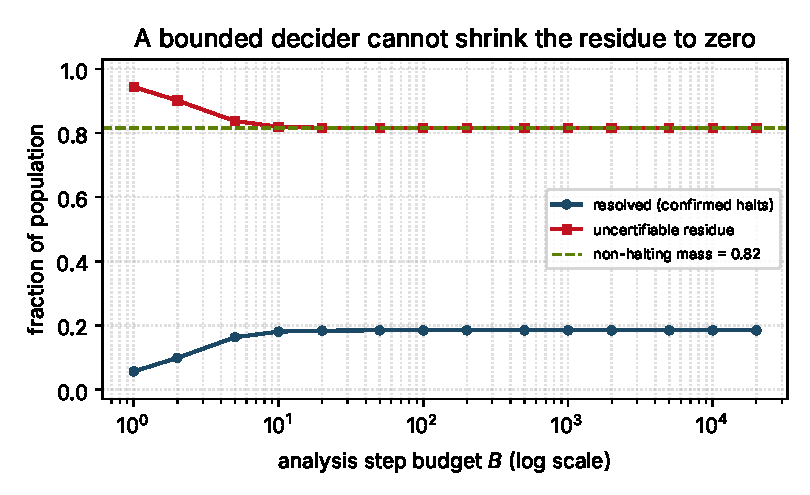
\includegraphics[width=0.82\linewidth]{results/figs/fig_residue.pdf}
  \caption{A bounded decider confirms the fast-halting minority almost
  immediately, but the residue it cannot certify safe does \emph{not} shrink to
  zero---it plateaus at the non-halting mass (\expNonhaltPct\%). More budget
  buys almost nothing past the knee. This is \Cref{prop:semidec} made visible.}
  \label{fig:residue}
\end{figure}

The shape is the point. Because halting (when it happens) happens early,
raising $B$ past a few dozen steps adds essentially no resolving power, yet the
residue stays at \expNonhaltPct\%. A sound agent is therefore \emph{cheap to
make confident about guilt and unable, at any price, to certify innocence} for
this population. Translated to security: a monitor can flag behaviour it
watches occur, but ``I ran it and saw nothing'' is not, and can never be
upgraded into, ``it is safe''.

\section{Study 2: Any Forced Decider Can Be Fooled}
\label{sec:study2}
Study 1 concerns a \emph{sound} agent that is allowed to abstain. Most deployed
agents are instead forced to emit a binary verdict. For such agents the dual
failure is available to the attacker: diagonalization.

\paragraph{Construction.}
Let $D$ be any total detector mapping program source to
$\{\textsc{mal},\textsc{ben}\}$. Define the \emph{evader} $E_D$ whose executed
semantics are
\[
  \textsc{behave}(E_D) \;=\;
  \begin{cases}
    \textsc{ben} & \text{if } D(\langle E_D\rangle)=\textsc{mal},\\
    \textsc{mal} & \text{if } D(\langle E_D\rangle)=\textsc{ben}.
  \end{cases}
\]
By construction $D$ is wrong about $E_D$. This is the same diagonal step as in
the halting proof and in Cohen's virus argument~\cite{cohen1987,chesswhite2000}.

\paragraph{Execution.}
We implement three detectors---a signature scanner, a suspicious-keyword
heuristic, and an entropy (``packed/obfuscated'') heuristic---and an
interpreter realising $\textsc{behave}(\cdot)$. For each detector we generate
\expEvaderM{} seeded evader variants (with randomised innocuous padding so the
detectors' verdicts genuinely vary), run each, and check the verdict against
the executed behaviour. Across all \expEvTrials{} trials the detector is wrong
every time: a \textbf{\expEvRate\% evasion rate} (\Cref{tab:evasion}). The
construction needs no knowledge of the detector's internals beyond oracle
access to its verdict---precisely what an adaptive adversary has.

\begin{table}[t]
  \centering
  \caption{Executed diagonalization. Each detector is queried as an oracle and
  misclassifies every constructed evader.}
  \label{tab:evasion}
  \begin{tabular}{lccc}
    \toprule
    Detector & Trials & Evasions & Rate \\
    \midrule
    Signature scanner      & \expEvaderM{} & \expEvaderM{} & 100\% \\
    Keyword heuristic      & \expEvaderM{} & \expEvaderM{} & 100\% \\
    Entropy heuristic      & \expEvaderM{} & \expEvaderM{} & 100\% \\
    \midrule
    \textbf{Total}         & \expEvTrials{} & \expEvTrials{} & \textbf{\expEvRate\%} \\
    \bottomrule
  \end{tabular}
\end{table}

The lesson is not that these particular heuristics are weak; it is that
\emph{oracle access to any fixed decider suffices to defeat it}. A more
powerful agent raises the attacker's constant factor, not the asymptotics.

\section{Study 3: Pricing the Trade-off Under a Real Adversary}
\label{sec:study3}
Soundness-with-abstention (Study 1) and forced-decision fragility (Study 2) are
the two theoretical poles. Real detonation/sandbox pipelines live in between:
they run a sample for a bounded \emph{analysis window} and flag it if malice
manifests. The adversary's countermeasure is timing---logic bombs, long sleeps,
environment-triggered payloads that simply outlast the window.

We model a population of \expSbN{} programs, \expSbBenignPct\% genuinely benign
(they never trigger) and the rest malicious with a trigger delay drawn from an
explicit heavy-tailed mixture (quick, delayed, and dormant components; median
delay \expSbMedDelay{} steps, $99$th percentile \expSbDelayTail{} steps). A sound
window of size $B$ catches a malicious sample iff its delay is $\le B$; benign
samples are never falsely flagged. \Cref{fig:sandbox} shows recall, false
negatives, and mean cost as $B$ grows.

\begin{figure}[t]
  \centering
  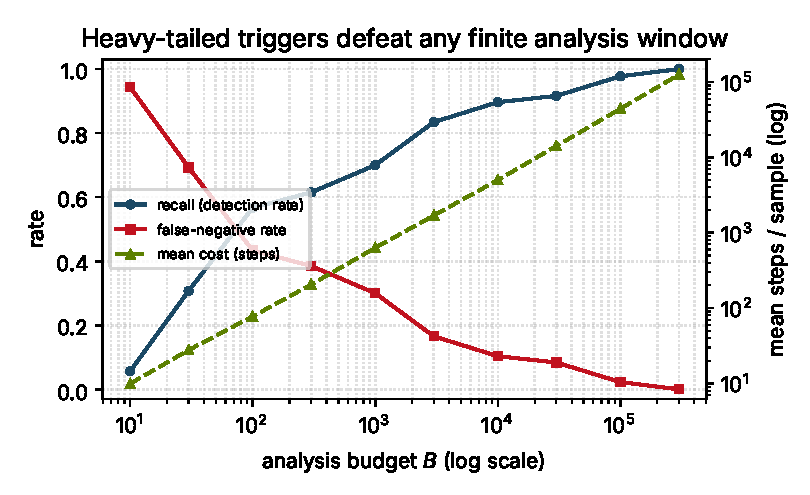
\includegraphics[width=0.82\linewidth]{results/figs/fig_sandbox.pdf}
  \caption{Recall rises with the analysis window but the heavy tail of trigger
  delays makes the final stretch brutally expensive: closing the last few
  percent of false negatives costs orders of magnitude more compute, and a
  dormant fraction outlasts any finite window.}
  \label{fig:sandbox}
\end{figure}

At a realistic \expSbWindow-step window the detector achieves \expSbRecall\%
recall---so \expSbFnr\% of malicious samples slip through purely by waiting. No
window size removes the tail: this is the budgeted, probabilistic shadow of
\Cref{prop:semidec} and of the \textsc{NP}-completeness of bounded
detection~\cite{spinellis2003}. An agent that reports ``\expSbRecall\% caught''
as ``safe'' is mistaking its budget for a proof.

\section{Discussion: Designing Agents That Know Their Limits}
\label{sec:discussion}
The results are negative about \emph{completeness}, not about usefulness. They
suggest a design posture.

\begin{itemize}[leftmargin=1.4em,itemsep=3pt]
  \item \textbf{Prefer soundness with explicit abstention.} Study 1 says an
  agent can be trustworthy about what it \emph{does} flag while being honest
  that silence is not safety. A third verdict---\textsc{undetermined}---is not
  a cop-out; it is the only truthful output for the residue.
  \item \textbf{Treat adaptive evasion as structural.} Study 2 says any fixed
  decider is defeatable by an adversary with oracle access. Defence should
  assume the attacker can query the agent and should diversify and randomise
  rather than trust a single frozen policy.
  \item \textbf{Budget is not proof.} Study 3 says recall figures are
  statements about an assumed delay distribution, not guarantees. Agents should
  publish their analysis budget and the evasion cost it implies, so a
  \expSbRecall\% number is read as ``under this budget and this threat model''.
  \item \textbf{Compose undecidable detection with decidable containment.}
  Because the verdict problem is undecidable, security should not rest on it
  alone: least privilege, capability confinement, and reversible actions turn
  a missed detection into a bounded loss rather than a breach.
\end{itemize}

\paragraph{Scope and limitations.}
Study 1's population is random Turing machines, not real software, and random
TMs halt early or not at all; the measured residue is an instance of the
asymmetry, not an estimate of real-world base rates. Study 3's numbers are
properties of a chosen distribution and should not be quoted as empirical
malware statistics. Study 2 is a constructive impossibility result; it says
nothing about how \emph{often} real attackers build such evaders, only that
they always can. None of the three weakens the central claim, which is a
statement about computation, not about any particular dataset.

\section{Related Work}
\label{sec:related}
The undecidability of detection traces to Turing~\cite{turing1936} and
Rice~\cite{rice1953}, applied to malicious code by Cohen~\cite{cohen1987} and
sharpened by Chess and White~\cite{chesswhite2000}; Spinellis~\cite{spinellis2003}
established \textsc{NP}-completeness of bounded-length virus identification. A
parallel literature studies the fragility of learned detectors under
adaptation: Barreno et al.~\cite{barreno2010} framed the security of machine
learning, and Biggio and Roli~\cite{biggiroli2018} traced a decade of evasion
and poisoning attacks; Goodfellow et al.~\cite{goodfellow2015} showed the ease
of adversarial examples. Our Study 2 connects that fragility back to its
computability-theoretic root: adaptive evasion is not merely empirically easy,
it is a diagonal argument. Sipser~\cite{sipser2013} is our standard reference
for the underlying theory.

\section{Conclusion}
\label{sec:conclusion}
Autonomous AI security agents are bounded deciders for undecidable problems. We
measured what that costs: a sound agent leaves an \expNonhaltPct\%
uncertifiable residue it can never close (Study 1); any forced decider is
defeated with \expEvRate\% reliability by a diagonal evader (Study 2); and a
realistic analysis window misses \expSbFnr\% of malicious samples to timing
alone (Study 3). The engineering response is not a better oracle---none exists.
It is to build agents that are sound, calibrated, and explicit about their
blind spots, and to pair undecidable detection with decidable containment. An
agent that knows what it cannot know is more secure than one that pretends to
know everything.

\begin{thebibliography}{99}
\bibitem{turing1936} A.~M. Turing, ``On Computable Numbers, with an
  Application to the Entscheidungsproblem,'' \emph{Proceedings of the London
  Mathematical Society}, ser.~2, vol.~42, pp.~230--265, 1936.
\bibitem{rice1953} H.~G. Rice, ``Classes of Recursively Enumerable Sets and
  Their Decision Problems,'' \emph{Transactions of the American Mathematical
  Society}, vol.~74, no.~2, pp.~358--366, 1953.
\bibitem{cohen1987} F.~Cohen, ``Computer Viruses: Theory and Experiments,''
  \emph{Computers \& Security}, vol.~6, no.~1, pp.~22--35, 1987.
\bibitem{chesswhite2000} D.~M. Chess and S.~R. White, ``An Undetectable
  Computer Virus,'' in \emph{Proceedings of the 2000 Virus Bulletin
  International Conference (VB2000)}, Orlando, FL, 2000.
\bibitem{spinellis2003} D.~Spinellis, ``Reliable Identification of
  Bounded-Length Viruses is NP-Complete,'' \emph{IEEE Transactions on
  Information Theory}, vol.~49, no.~1, pp.~280--284, 2003.
\bibitem{sipser2013} M.~Sipser, \emph{Introduction to the Theory of
  Computation}, 3rd~ed. Boston, MA: Cengage Learning, 2013.
\bibitem{barreno2010} M.~Barreno, B.~Nelson, A.~D. Joseph, and J.~D. Tygar,
  ``The Security of Machine Learning,'' \emph{Machine Learning}, vol.~81,
  no.~2, pp.~121--148, 2010.
\bibitem{biggiroli2018} B.~Biggio and F.~Roli, ``Wild Patterns: Ten Years
  After the Rise of Adversarial Machine Learning,'' \emph{Pattern Recognition},
  vol.~84, pp.~317--331, 2018.
\bibitem{goodfellow2015} I.~J. Goodfellow, J.~Shlens, and C.~Szegedy,
  ``Explaining and Harnessing Adversarial Examples,'' in \emph{International
  Conference on Learning Representations (ICLR)}, 2015.
\end{thebibliography}

\end{document}
